% !TeX spellcheck = pt-br
\documentclass[12pt, a4paper, portuguese]{fphw}
\usepackage[utf8]{inputenc}
\usepackage[T1]{fontenc}
\usepackage[brazil]{babel}
\usepackage{mathpazo}
\usepackage{graphicx}
\usepackage{booktabs}
\usepackage{listings} % Required for insertion of code
\usepackage{enumerate}
\usepackage{amsmath}
\usepackage{float}

\usepackage{hyperref}
\hypersetup{
	colorlinks=true,
	linkcolor=blue,
	filecolor=magenta,      
	urlcolor=blue,
}

\title{
	Projeto de Estudos
}

\author{Myke Albuquerque Pinto de Oliveira}
\institute{UnisulVirtual \\ Universidade do Sul de Santa Catarina}
\class{Equações Diferenciais Parciais}
\professor{Christian Wagner}
\date{4 de novembro de 2020}

\DeclareMathOperator{\sen}{sen}
\DeclareMathOperator{\senh}{senh}

\begin{document}

\maketitle

\part{Equação da Onda}

\section*{Problema 10}

\begin{problem}
	Considere uma corda elástrica de comprimento $ L $. A extremidade $ x = 0 $ é mantida fixa enquanto a extremidade $ x = L $ está solta; assim, as condições de contorno são $ u(0, t) = 0 $ e $ u(L, t) = 0 $. A corda é colocada em movimento, sem velocidade inicial, a partir da posição inicial $ u(x, 0) = f(x) $, em que
	
	$$
	f(x) = \begin{cases}
	1, \, L/2 - 1 < x < L/2 + 1 \, (L > 2), \\
	0 \textrm{ caso contrário.}
	\end{cases}
	$$
	
	\begin{enumerate}[(a)]
		
		\item Calcule o deslocamento $ u(x, t) $.
		
		\item Com $ L = 10 $ e $ a = 1 $, faça o gráfico de $ u $ em função de $ x $ para $ 0 \le x \le 10 $ e para diversos valores de t. Preste atenção especial aos valores de $ t $ entre $ 3 $ e $ 7 $. Note como a perturbação inicial é refletida em cada extremidade da corda.
		
		\item Com $ L = 10 $ e $ a = 1 $, faça o gráfico de $ u $ em função de $ t $ para diversos valores de $ x $.
		
		\item Construa uma animação da solução no tempo durante pelo menos um período.
		
		\item Descreva o movimento da corda em algumas frases.
		
	\end{enumerate}
\end{problem}

%------------------------------------------------

\subsection*{Resposta}

Em primeiro lugar, vamos resolver a EDP da onda $ a^2 u_{xx} = u_tt $. Usando o método da separação de variáveis, vamos tentar a solução $ u(x, t) = X(x) \cdot T(t) $. Aplicando na EDP, tem-se:

$$
a^2 X''(x) \cdot T(t) = X(x) \cdot T''(t)
$$

$$
\frac{X''(x)}{X(x)} = \frac{1}{a^2} \frac{T''(t)}{T(t)}
$$

$$
\begin{cases}
\frac{X''(x)}{X(x)} = -\lambda \\
\frac{1}{a^2} \frac{T''(t)}{T(t)} = -\lambda
\end{cases}
$$

$$
\begin{cases}
X''(x) + \lambda X(x) = 0 \\
T''(t) + a^2 \lambda T(t) = 0
\end{cases}
$$

Caso $ \lambda < 0 $:

$$
X(x) = Ae^{\sqrt{-\lambda}x} + Be^{-\sqrt{-\lambda}x}
$$

$$
T(t) = Ce^{a\sqrt{-\lambda}t} + De^{-a\sqrt{-\lambda}t}
$$

Impondo a condição de contorno:

$$
u(0, t) = X(0)T(t) = (A + B) (Ce^{\sqrt{-\lambda}t} + De^{-\sqrt{-\lambda}t})
$$

Isso implica $ A + B = 0 $ ou $ C = 0 $ e $ D = 0 $, ou seja, a solução trivial, a qual não estamos interessados.

Caso $ \lambda = 0 $:

$$
X(x) = Ax + B
$$

$$
T(t) = Ct + D
$$

Impondo as condições de contorno:

$$
u(0, t) = X(0)T(t) = B(Ct + D) = 0
$$

O que também acarreta na solução trivial.

Caso $ \lambda > 0 $:

$$
X(x) = A \sen \left( \sqrt{-\lambda} x \right) + B \cos \left( \sqrt{-\lambda} x \right)
$$

$$
T(t) = C \sen \left( a\sqrt{-\lambda} t \right) + D \cos \left( a\sqrt{-\lambda} t \right)
$$

Impondo as condições de contorno:

$$
u(0, t) = \left[
A \sen \left( \sqrt{-\lambda} x \right) + B \cos \left( \sqrt{-\lambda} x \right)
\right]_{x=0}
\cdot
\left[
C \sen \left( a\sqrt{-\lambda} t \right) + D \cos \left( a\sqrt{-\lambda} t \right)
\right] = 0
$$

$$
u(0, t) = B
\left[
C \sen \left( a\sqrt{-\lambda} t \right) + D \cos \left( a\sqrt{-\lambda} t \right)
\right]
$$

$$
B = 0
$$

$$
u(L, t) = \left[
A \sen \left( \sqrt{-\lambda} x \right)
\right]_{x=L}
\cdot
\left[
C \sen \left( a\sqrt{-\lambda} t \right) + D \cos \left( a\sqrt{-\lambda} t \right)
\right] = 0
$$

$$
u(L, t) = \left[
A \sen \left( \sqrt{-\lambda} L \right)
\right]
\cdot
\left[
C \sen \left( a\sqrt{-\lambda} t \right) + D \cos \left( a\sqrt{-\lambda} t \right)
\right] = 0
$$

Para algum $ n $ natural:

$$
\sqrt{-\lambda} L = n \pi
$$

$$
\sqrt{-\lambda} = \frac{n \pi}{L}
$$

E a condição inicial de velocidade nula:

$$
u_t(x, 0) = \left[
A \sen \left( \frac{n \pi}{L} x \right)
\right]
\cdot \left[
C a\frac{n \pi}{L} \cos \left( a\frac{n \pi}{L} t \right) + Da\frac{n \pi}{L} \sen \left( a\frac{n \pi}{L} t \right)
\right]_{t=0}
= 0
$$

$$
u_t(x, 0) = \left[
A \sen \left( \frac{n \pi}{L} x \right)
\right]
\cdot \left[
C a\frac{n \pi}{L}
\right]
= 0
$$

$$
C = 0
$$

Reescrevendo $ u(x, t) $:

$$
u(x, t) = \left[
A \sen \left( \frac{n \pi}{L} x \right)
\right]
\cdot
\left[
D \cos \left( a\frac{n \pi}{L} t \right)
\right]
$$

$$
u(x, t) =
AD \sen \left( \frac{n \pi}{L} x \right)
\cdot
\cos \left( a\frac{n \pi}{L} t \right)
$$

Definindo $ b_n = AD $, tem-se uma solução para cada natural $ n $.

$$
u_n(x, t) =
b_n \sen \left( \frac{n \pi}{L} x \right)
\cdot
\cos \left( a\frac{n \pi}{L} t \right)
$$

Vamos procurar por uma solução que satisfaça a condição inicial de posição a partir da combinação destas soluções já encontradas.

$$
u(x, t) = \sum_{n=1}^{\infty}
b_n \sen \left( \frac{n \pi}{L} x \right)
\cdot
\cos \left( a\frac{n \pi}{L} t \right)
$$

Impondo a condição inicial:

$$
u(x, 0) = \sum_{n=1}^{\infty}
b_n \sen \left( \frac{n \pi}{L} x \right)
= f(x)
$$

Os termos da série de Fourier são dados por:

$$
b_n = \frac{1}{L} \int_{-L}^{L} f(x) \sen \left( \frac{n\pi x}{L}\right)\, dx
$$

$$
b_n = \frac{2}{L} \int_{0}^{L} f(x) \sen \left( \frac{n\pi x}{L}\right)\, dx
$$

$$
b_n = \frac{2}{L} \int_{L/2-1}^{L/2+1} \sen \left( \frac{n\pi x}{L}\right)\, dx
$$

$$
b_n = \frac{2}{L} \left[ -\frac{L}{n\pi}\cos \left( \frac{n\pi x}{L}\right) \right]_{L/2-1}^{L/2+1}
$$

$$
b_n = -\frac{2}{n\pi} \left[\cos \left( \frac{n\pi x}{L}\right) \right]_{L/2-1}^{L/2+1}
$$

$$
b_n = -\frac{2}{n\pi} \left[\cos \left( \frac{n\pi (L/2+1)}{L}\right) - \cos \left( \frac{n\pi (L/2-1)}{L}\right) \right]
$$

$$
b_n = -\frac{2}{n\pi} \left[\cos \left( \frac{n\pi}{2} + \frac{n \pi}{L} \right) - \cos \left( \frac{n\pi}{2} - \frac{n \pi}{L} \right) \right]
$$

$$
b_n = -\frac{2}{n\pi} \left[
\cos \left( \frac{n\pi}{2} \right) \cos \left( \frac{n \pi}{L} \right)
-
\sen \left( \frac{n\pi}{2} \right) \sen \left( \frac{n \pi}{L} \right)
-
\cos \left( \frac{n\pi}{2} \right) \cos \left( \frac{n \pi}{L} \right)
-
\sen \left( \frac{n\pi}{2} \right) \sen \left( \frac{n \pi}{L} \right)
\right]
$$

$$
b_n = \frac{4}{n\pi} \left[
\sen \left( \frac{n\pi}{2} \right) \sen \left( \frac{n \pi}{L} \right)
\right]
$$

Explicitando a solução:

$$
u(x, t) = \sum_{n=1}^{\infty} b_n \sen \left( \frac{n \pi}{L} x \right)
\cdot
\cos \left( a\frac{n \pi}{L} t \right)
$$

$$
b_n = \begin{cases}
\frac{4}{n\pi} \sen \left( \frac{n \pi}{L} \right), &n \equiv 1 \mod 4 \\
0,                               &n \equiv 2 \vee n \equiv 0 \mod 4 \\
-\frac{4}{n\pi} \sen \left( \frac{n \pi}{L} \right), &n \equiv 3 \mod 4 
\end{cases}
$$

Seguem os gráficos para vários valores de t:

\begin{figure}[H]
	\centering
	\includegraphics[width=.8\linewidth]{"graficos/grafico_t=0.000s"}
	\caption{Onda na corda elástica no instante t=0.000s}
	\label{fig:grafico-t0}
\end{figure}

\begin{figure}[H]
	\centering
	\includegraphics[width=.8\linewidth]{"graficos/grafico_t=1.000s"}
	\caption{Onda na corda elástica no instante t=1.000s}
	\label{fig:grafico-t1}
\end{figure}

\begin{figure}[H]
	\centering
	\includegraphics[width=.8\linewidth]{"graficos/grafico_t=2.000s"}
	\caption{Onda na corda elástica no instante t=2.000s}
	\label{fig:grafico-t2}
\end{figure}

\begin{figure}[H]
	\centering
	\includegraphics[width=.8\linewidth]{"graficos/grafico_t=3.000s"}
	\caption{Onda na corda elástica no instante t=3.000s}
	\label{fig:grafico-t3}
\end{figure}

\begin{figure}[H]
	\centering
	\includegraphics[width=.8\linewidth]{"graficos/grafico_t=3.500s"}
	\caption{Onda na corda elástica no instante t=3.500s}
	\label{fig:grafico-t3.5}
\end{figure}

\begin{figure}[H]
	\centering
	\includegraphics[width=.8\linewidth]{"graficos/grafico_t=4.000s"}
	\caption{Onda na corda elástica no instante t=4.000s}
	\label{fig:grafico-t4}
\end{figure}

\begin{figure}[H]
	\centering
	\includegraphics[width=.8\linewidth]{"graficos/grafico_t=4.500s"}
	\caption{Onda na corda elástica no instante t=4.500s}
	\label{fig:grafico-t4.5}
\end{figure}

\begin{figure}[H]
	\centering
	\includegraphics[width=.8\linewidth]{"graficos/grafico_t=5.000s"}
	\caption{Onda na corda elástica no instante t=5.000s}
	\label{fig:grafico-t5}
\end{figure}

\begin{figure}[H]
	\centering
	\includegraphics[width=.8\linewidth]{"graficos/grafico_t=5.500s"}
	\caption{Onda na corda elástica no instante t=5.500s}
	\label{fig:grafico-t5.5}
\end{figure}

\begin{figure}[H]
	\centering
	\includegraphics[width=.8\linewidth]{"graficos/grafico_t=6.000s"}
	\caption{Onda na corda elástica no instante t=6.000s}
	\label{fig:grafico-t6}
\end{figure}

\begin{figure}[H]
	\centering
	\includegraphics[width=.8\linewidth]{"graficos/grafico_t=6.500s"}
	\caption{Onda na corda elástica no instante t=6.500s}
	\label{fig:grafico-t6.5}
\end{figure}

\begin{figure}[H]
	\centering
	\includegraphics[width=.8\linewidth]{"graficos/grafico_t=7.000s"}
	\caption{Onda na corda elástica no instante t=7.000s}
	\label{fig:grafico-t7}
\end{figure}

Seguem agora os gráficos da onda em função de $ t $ para vários $ x $'s.

\begin{figure}[H]
	\centering
	\includegraphics[width=.8\linewidth]{"graficos/grafico_x=0.000m"}
	\caption{Onda na corda elástica na cota x=0.000m}
	\label{fig:grafico-x0}
\end{figure}

\begin{figure}[H]
	\centering
	\includegraphics[width=.8\linewidth]{"graficos/grafico_x=1.000m"}
	\caption{Onda na corda elástica na cota x=1.000m}
	\label{fig:grafico-x1}
\end{figure}

\begin{figure}[H]
	\centering
	\includegraphics[width=.8\linewidth]{"graficos/grafico_x=2.000m"}
	\caption{Onda na corda elástica na cota x=2.000m}
	\label{fig:grafico-x2}
\end{figure}

\begin{figure}[H]
	\centering
	\includegraphics[width=.8\linewidth]{"graficos/grafico_x=3.000m"}
	\caption{Onda na corda elástica na cota x=3.000m}
	\label{fig:grafico-x3}
\end{figure}

\begin{figure}[H]
	\centering
	\includegraphics[width=.8\linewidth]{"graficos/grafico_x=4.000m"}
	\caption{Onda na corda elástica na cota x=4.000m}
	\label{fig:grafico-x4}
\end{figure}

\begin{figure}[H]
	\centering
	\includegraphics[width=.8\linewidth]{"graficos/grafico_x=5.000m"}
	\caption{Onda na corda elástica na cota x=5.000m}
	\label{fig:grafico-x5}
\end{figure}

\begin{figure}[H]
	\centering
	\includegraphics[width=.8\linewidth]{"graficos/grafico_x=6.000m"}
	\caption{Onda na corda elástica na cota x=6.000m}
	\label{fig:grafico-x6}
\end{figure}

\begin{figure}[H]
	\centering
	\includegraphics[width=.8\linewidth]{"graficos/grafico_x=7.000m"}
	\caption{Onda na corda elástica na cota x=7.000m}
	\label{fig:grafico-x7}
\end{figure}

\begin{figure}[H]
	\centering
	\includegraphics[width=.8\linewidth]{"graficos/grafico_x=8.000m"}
	\caption{Onda na corda elástica na cota x=8.000m}
	\label{fig:grafico-x8}
\end{figure}

\begin{figure}[H]
	\centering
	\includegraphics[width=.8\linewidth]{"graficos/grafico_x=9.000m"}
	\caption{Onda na corda elástica na cota x=9.000m}
	\label{fig:grafico-x9}
\end{figure}

\begin{figure}[H]
	\centering
	\includegraphics[width=.8\linewidth]{"graficos/grafico_x=10.000m"}
	\caption{Onda na corda elástica na cota x=10.000m}
	\label{fig:grafico-x10}
\end{figure}

A simulação animada está disponível em \url{https://youtu.be/wT0QXQl6sjE}.

Podemos perceber que a perturbação inicial se divide igualmente e se propaga para cada um dos lados. Ao atingir uma extremidade fixa, a perturbação reflete em oposição de fase, interferindo em si própria e quano os pulsos se encontram forma uma interferência construtiva aumentando sua intensidade.

\part{Equação de Laplace}

\section*{Problema 12}

\begin{problem}
	\begin{enumerate}[(a)]
		
		\item Encontre a solução $ u(x, y) $ da equação de Laplace no retângulo $ 0 < x < a, 0 < y < b $, que satisfaz as condições de contorno
		
		$$
		\begin{aligned}
			u(0, y)   &= 0, & u(a, y) &= 0,    & 0 < y < b, \\
			u_y(x, 0) &= 0, & u(x, b) &= g(x), & 0 \le x \le a.
		\end{aligned}
		$$
		
		Note que esse não é um problema de Dirichlet nem de Neumann, mas um problema misto no qual $ u $ é dada em parte da fronteira e sua derivada normal é dada no resto.
		
		\item Encontre a solução se
		
		$$
		g(x) = \begin{cases}
		x,     & 0 \le x \le a/2, \\
		a - x, & a/2 \le x \le a
		\end{cases}
		$$
		
		\item Sejam $ a = 3 $ e $ b = 1 $. Fazendo gráficos apropriados, compare essa solução com a do Problema 1.
		
	\end{enumerate}
\end{problem}

\subsection*{Resposta}

$$
\nabla^2 u = 0
$$

$$
u_{xx} + u_{yy} = 0
$$

Tomando $ u(x, y) = X(x) \cdot Y(y) $.

$$
X''(x) \cdot Y(y) + X(x) \cdot Y''(y) = 0
$$

$$
X''(x) \cdot Y(y) = -X(x) \cdot Y''(y)
$$

$$
\frac{X''(x)}{X(x)} = - \frac{Y''(y)}{Y(y)}
$$

$$
\begin{cases}
\frac{X''(x)}{X(x)} = - \lambda \\
\frac{Y''(y)}{Y(y)} = \lambda
\end{cases}
$$

$$
\begin{cases}
X''(x) + \lambda X(x) = 0 \\
Y''(y) - \lambda Y(y) = 0
\end{cases}
$$

Caso $ \lambda < 0 $:

$$
X(x) = A e^{\sqrt{-\lambda} x} + B e^{\sqrt{-\lambda} x}
$$

$$
Y(y) = C \cos \left( \sqrt{-\lambda} y \right) + D \sen \left( \sqrt{-\lambda} y \right)
$$

Impondo a condição $ u(0, y) = 0 $ implica na solução trivial.

Caso $ \lambda = 0 $:

$$
X(x) = Ax + B
$$

$$
Y(y) = Cy + D
$$

Impondo a condição $ u(0, y) = 0 $ e $ u(a, y) = 0 $ implica na solução trivial.

Caso $ \lambda > 0 $:

$$
X(x) = A \cos \left( \sqrt{\lambda} x \right) + B \sen \left( \sqrt{\lambda} x \right)
$$

$$
Y(y) = C e^{\sqrt{\lambda} y} + D e^{-\sqrt{\lambda} y}
$$

Impondo a condição $ u(0, y) = 0 $, implica que $ A = 0 $, e impondo $ u(a, y) = 0 $, implica em $ \sqrt{\lambda} a = n \pi \rightarrow \sqrt{\lambda} = \frac{n \pi}{a} $ para algum $ n $ natural.

$$
X(x) = B \sen \left( \frac{n \pi}{a} x \right)
$$

$$
Y(y) = C e^{\frac{n \pi}{a} y} + D e^{\frac{n \pi}{a} y}
$$

$$
Y'(y) = C \frac{n \pi}{a} e^{\frac{n \pi}{a} y} - D \frac{n \pi}{a} e^{-\frac{n \pi}{a} y}
$$

Impondo a condição de contorno $ u_y(x, 0) = 0 $, tem-se:

$$
C \frac{n \pi}{a} - D \frac{n \pi}{a} = 0
$$

$$
C = D
$$

O que resulta na solução para um $ n $ particular:

$$
u_n(x, y) = \left[
 B \sen \left( \frac{n \pi}{a} x \right)
\right]
\cdot
\left[
C \senh \left(
\frac{n \pi}{a} y
\right)
\right]
$$

$$
u_n(x, y) =
a_n \sen \left( \frac{n \pi}{a} x \right)
\cdot
\senh \left(
\frac{n \pi}{a} y
\right)
$$

$$
u(x, y) = \sum_{n=1}^{\infty}
a_n \sen \left( \frac{n \pi}{a} x \right)
\cdot
\senh \left(
\frac{n \pi}{a} y
\right)
$$

Impondo a condição de contorno $ u(x, b) = g(x) $, tem-se:

$$
\sum_{n=1}^{\infty}
a_n \sen \left( \frac{n \pi}{a} x \right)
\cdot
\senh \left(
\frac{n \pi}{a} b
\right) = g(x)
$$

Os coeficientes da série de Fourier são:

$$
a_n
\senh \left(
\frac{n \pi}{a} b
\right)
=
\frac{1}{a} \int_{-a}^{a} g(x) \sen \left( \frac{n \pi}{a} x \right)\, dx
$$

$$
a_n
=
\frac{1}{a \senh \left(
\frac{n \pi}{a} b
\right)} \int_{-a}^{a} g(x) \sen \left( \frac{n \pi}{a} x \right)\, dx
$$

Explicitando a solução, tem-se:

$$
u(x, y) = \sum_{n=1}^{\infty}
\frac{1}{a \senh \left(
\frac{n \pi}{a} b
\right)} \int_{-a}^{a} g(x) \sen \left( \frac{n \pi}{a} x \right)\, dx
\sen \left( \frac{n \pi}{a} x \right)
\cdot
\senh \left(
\frac{n \pi}{a} y
\right)
$$

Vamos agora tomar a solução dada no item (b).
$$
\begin{aligned}
\int_{-a}^{a} g(x) \sen \left( \frac{n \pi}{a} x \right)\, dx
&= 2\int_{0}^{a} g(x) \sen \left( \frac{n \pi}{a} x \right)\, dx \\
&= 2 \left(
\int_{0}^{a/2} x \sen \left( \frac{n \pi}{a} x \right)\, dx
+
\int_{a/2}^{a} \left( a - x \right) \sen \left( \frac{n \pi}{a} x \right)\, dx
\right)
\end{aligned}
$$

$$
\begin{aligned}
\int_{0}^{a/2} x \sen \left( \frac{n \pi}{a} x \right)\, dx
&=
\left[
-\frac{a}{n \pi}x
\cos \left( \frac{n\pi}{a}x \right)
+
\frac{a^2}{n^2 \pi^2}
\sen \left( \frac{n\pi}{a}x \right)
\right]_0^{a/2} \\
&=
-\frac{a^2}{2n \pi}
\cos \left( \frac{n\pi}{2} \right)
+
\frac{a^2}{n^2 \pi^2}
\sen \left( \frac{n\pi}{2} \right)
\end{aligned}
$$

$$
\begin{aligned}
\int_{a/2}^{a} \left( a - x \right) \sen \left( \frac{n \pi}{a} x \right)\, dx &= \int_{a/2}^{a} a \sen \left( \frac{n \pi}{a} x \right)\, dx - \int_{a/2}^{a} x \sen \left( \frac{n \pi}{a} x \right)\, dx \\
&=
\left[
-\frac{a^2}{n\pi} \cos \left( \frac{n \pi}{a} x \right)
+\frac{a}{n \pi}x
\cos \left( \frac{n\pi}{a}x \right)
-
\frac{a^2}{n^2 \pi^2}
\sen \left( \frac{n\pi}{a}x \right)
\right]_{a/2}^a \\
&=
-\frac{a^2}{n\pi} \cos \left( n \pi \right)
+\frac{a^2}{n \pi}
\cos \left( n\pi \right)
-
\frac{a^2}{n^2 \pi^2}
\sen \left( n\pi \right) \\
&+
\frac{a^2}{n\pi} \cos \left( \frac{n \pi}{2} \right)
-\frac{a^2}{2n \pi}
\cos \left( \frac{n\pi}{2} \right)
+
\frac{a^2}{n^2 \pi^2}
\sen \left( \frac{n\pi}{2} \right) \\
&=
\frac{a^2}{2n\pi} \cos \left( \frac{n \pi}{2} \right)
+
\frac{a^2}{n^2 \pi^2}
\sen \left( \frac{n\pi}{2} \right) \\
\end{aligned}
$$

$$
\begin{aligned}
\int_{-a}^{a} g(x) \sen \left( \frac{n \pi}{a} x \right)\, dx
=
2
\left(
-\frac{a^2}{2n \pi}
\cos \left( \frac{n\pi}{2} \right)
+
\frac{a^2}{n^2 \pi^2}
\sen \left( \frac{n\pi}{2} \right)
+
\frac{a^2}{2n\pi} \cos \left( \frac{n \pi}{2} \right)
+
\frac{a^2}{n^2 \pi^2}
\sen \left( \frac{n\pi}{2} \right)
\right)
\end{aligned}
$$

$$
\begin{aligned}
\int_{-a}^{a} g(x) \sen \left( \frac{n \pi}{a} x \right)\, dx
=
2
\left(
\frac{a^2}{n^2 \pi^2}
\sen \left( \frac{n\pi}{2} \right)
+
\frac{a^2}{n^2 \pi^2}
\sen \left( \frac{n\pi}{2} \right)
\right)
\end{aligned}
$$

$$
\int_{-a}^{a} g(x) \sen \left( \frac{n \pi}{a} x \right)\, dx
=
\frac{4a^2}{n^2 \pi^2}
\sen \left( \frac{n\pi}{2} \right)
$$

A solução completa:

$$
u(x, y) = \sum_{n=1}^{\infty}
\frac{1}{a \senh \left(
	\frac{n \pi}{a} b
	\right)} \frac{4a^2}{n^2 \pi^2} \sen \left( \frac{n\pi}{2} \right)
\sen \left( \frac{n \pi}{a} x \right)
\cdot
\senh \left(
\frac{n \pi}{a} y
\right)
$$

\begin{figure}[H]
	\centering
	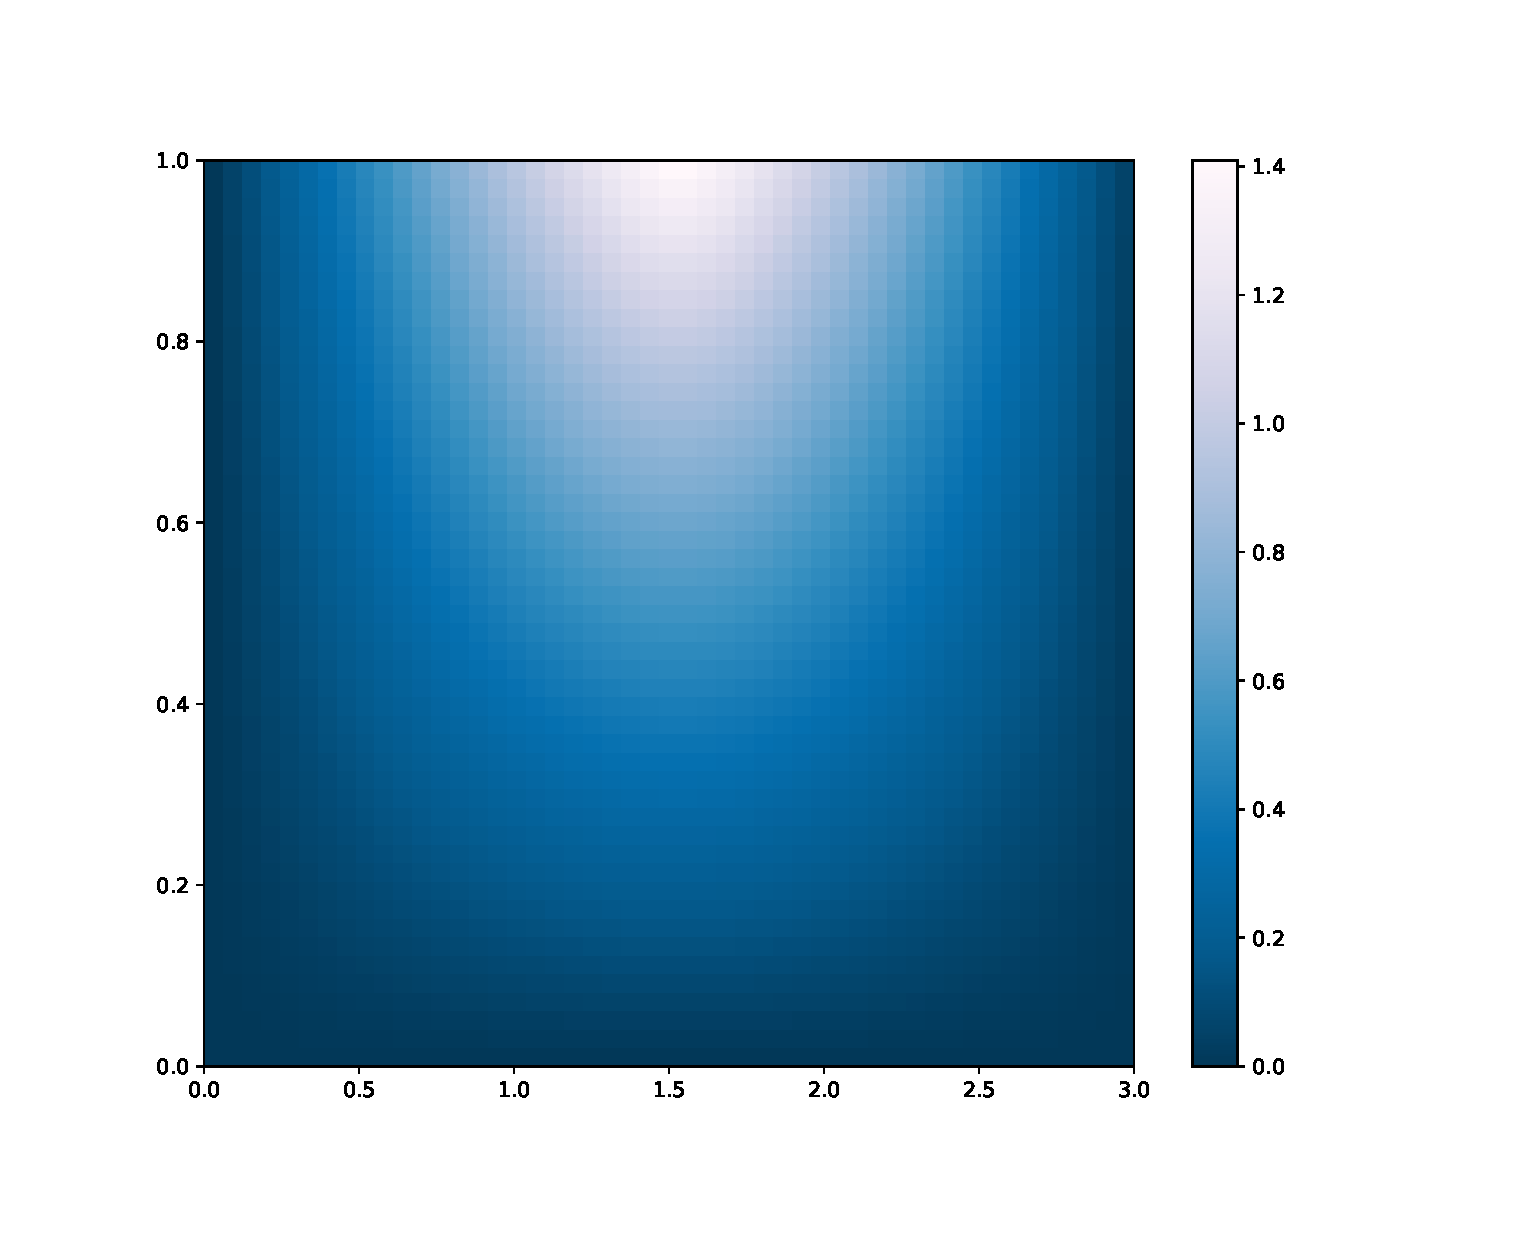
\includegraphics[width=1\linewidth]{graficos/mapadecalor}
	\caption{Representação da solução em tons de azul}
	\label{fig:mapadecalor}
\end{figure}

\begin{figure}[H]
	\centering
	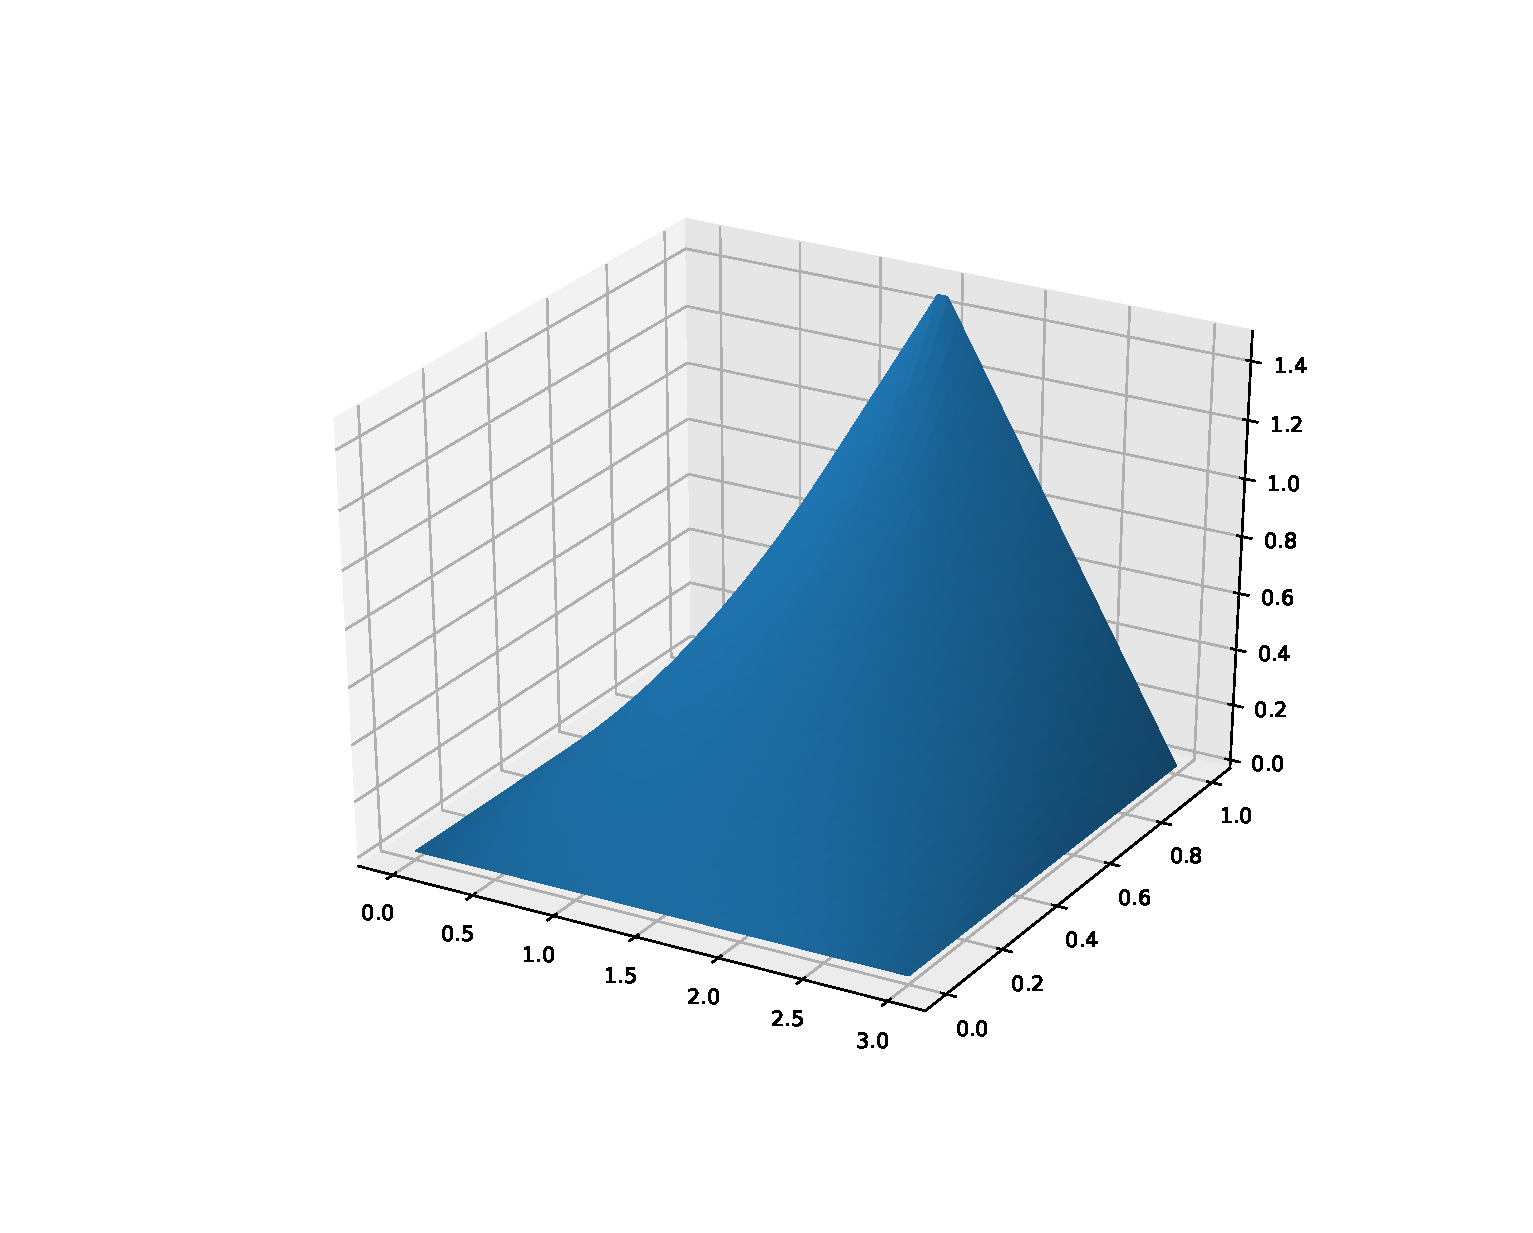
\includegraphics[width=1\linewidth]{graficos/problema2-3d}
	\caption{Representação em superfície da solução}
	\label{fig:problema2-3d}
\end{figure}



\end{document}